\documentclass[11pt,a4paper]{article}
\usepackage[utf8]{inputenc}
\usepackage[T1]{fontenc}
\usepackage{amsmath,amssymb}
\usepackage[margin=2.5cm]{geometry}
\usepackage{xcolor}
\usepackage{graphicx}

\setlength{\parindent}{0pt}
\setlength{\parskip}{6pt}

\begin{document}

\begin{center}
{\large Technical Neural Networks Assignment Sheet 4}\\[4pt]
{\bfseries Names: Mohamadhosein Sabaghi (50547423)}
\end{center}

\section*{Assignment 16}

With single-step (online) learning, one pattern $p$ is picked and the weights are updated right
after it, so the plotted error ${}^pE$ is the error of whichever single pattern was just shown --
not the total error over all patterns. That makes the curve inherently noisy: it jumps up and
down from step to step depending on how well the network currently happens to fit that
particular pattern, while only the underlying \emph{trend} decreases smoothly. Typical shape:

\begin{itemize}
  \item a fast drop at the very start, while the (randomly initialized) weights are still far from
  any reasonable solution;
  \item a longer middle phase where the trend keeps decreasing, but individual steps fluctuate a
  lot around it -- "hard" or just-updated-against patterns still produce temporary error spikes;
  \item a late phase where the trend flattens out near a low floor (ideally near $0$, or above $0$ if
  the task isn't perfectly learnable), with the step-to-step noise still visible on top of it --
  single-step learning never fully smooths out, unlike cumulative/batch learning (assignment 15).
\end{itemize}

\begin{center}
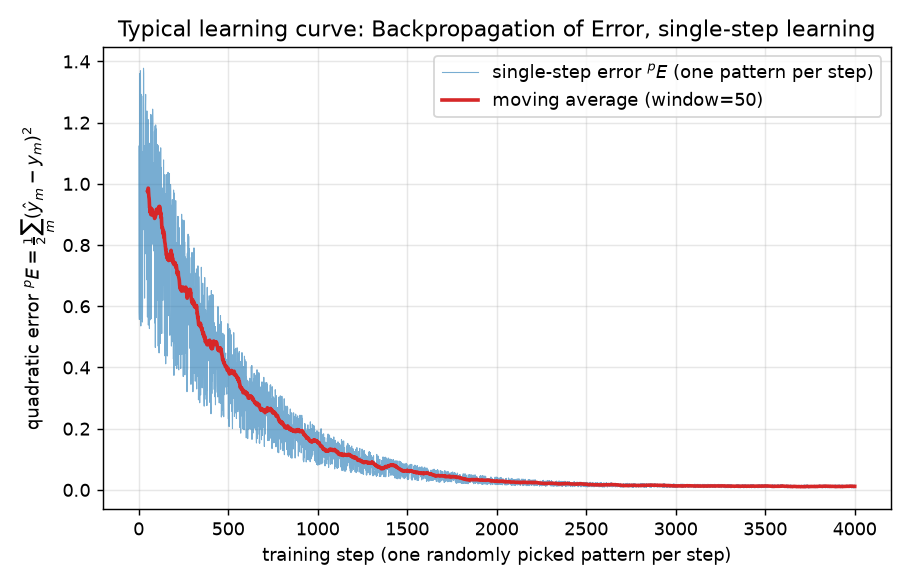
\includegraphics[width=0.85\textwidth]{learning_curve_typical.png}
\end{center}

This matches what we actually observed empirically with our own single-step-trained MLPs in
PA-A (e.g.\ \texttt{assignments/2/pa\_a/data/01/learning\_curve.png}), and the real measured
example shown in the lecture: a steep early drop followed by a noisy decreasing trend that
settles near a low error floor.

\section*{Assignment 17}

$f(z) = 2^{\,2-z+4\sin(z)}$, plotted over $z\in[0.05,12]$ in the 4 required scalings:

\begin{center}
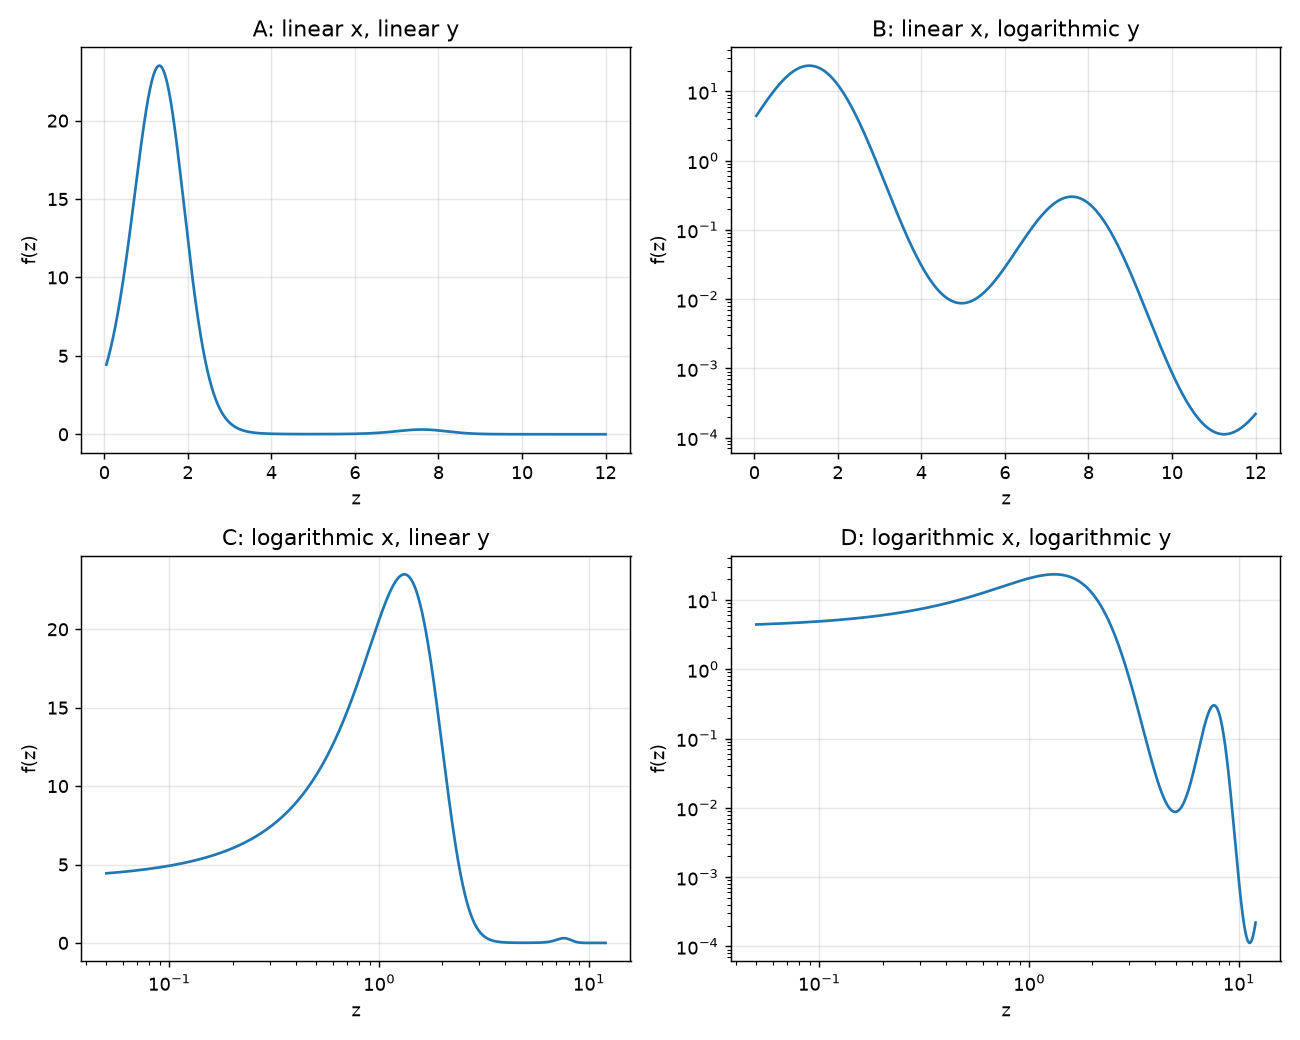
\includegraphics[width=\textwidth]{log_scale_demo.png}
\end{center}

$f(z)$ ranges from about $1\!\times\!10^{-4}$ to $24$ here -- five orders of magnitude -- which is
exactly what makes the different scalings behave so differently:

\begin{itemize}
  \item \textbf{A (linear/linear):} shows the true values, but the huge early peak dominates the
  plot and squashes everything else onto the $x$-axis. The secondary bump around $z\approx7.5$ and
  the late uptick near $z\approx11.5$ are completely invisible. For a real learning curve this is
  dangerous -- it would hide whether training has actually converged, or is still slowly moving
  (or relapsing) at low error.
  \item \textbf{B (linear $z$, logarithmic $f$):} this is how learning curves are normally plotted
  (as in the lecture). Every order of magnitude gets the same vertical space, so the secondary
  bump, the dip, and the late uptick all become clearly visible. Since errors often decay roughly
  exponentially, this also tends to turn the decay into a close-to-straight line, making the decay
  rate and deviations from it (plateaus, local minima) easy to read off.
  \item \textbf{C (logarithmic $z$, linear $f$):} stretches out the early part of training (small
  $z$) and compresses the long tail -- useful when the early dynamics matter most -- but the $y$-axis
  is still linear, so it suffers from the same problem as A: small late-stage values are invisible.
  \item \textbf{D (log/log):} combines both effects -- the late-stage structure is visible like in
  B, and the early part is stretched out like in C. A straight line in a log-log plot would
  indicate a power-law decay; this curve is not straight, confirming the decay here isn't a pure
  power law.
\end{itemize}

\section*{Assignment 18}

\textbf{8-3-8.} The input is an 8-bit 1-out-of-8 vector, and the teacher equals the input (an
autoencoder task). There are only 8 possible input patterns, and with 3 hidden neurons we can
represent exactly $2^3=8$ distinct binary codes -- so the hidden layer can learn one (near-saturated)
code per pattern, and the output layer can decode each code back to the right 1-out-of-8 pattern.
The invented code doesn't have to match ``normal'' binary counting, it only needs 8 codes that
are distinguishable from each other.

\textbf{8-2-8.} Only 2 bits seems too few ($2^2=4<8$), but the hidden neurons aren't restricted to
exactly $0/1$ -- they output continuous real values, so the pair $(\mathrm{out}_{h1},\mathrm{out}_{h2})$
can be any point in a 2D region. The connection from hidden to output layer is just a (single-layer)
Perceptron, which can only realize a \emph{linear} separation. So the task becomes: can the 8 codes
be placed in the 2D plane such that each one is linearly separable from the other 7 (so each output
neuron can fire for exactly its own code)? Yes -- placing the 8 codes at the vertices of a convex
polygon (e.g.\ evenly spaced on a circle) works, since any single vertex of a convex polygon can be
cut off from all the others by one straight line (a tangent/supporting line at that vertex).

\textbf{8-1-8 is not solvable.} With only 1 hidden neuron, the hidden ``space'' is just a single real
number $\mathrm{out}_{h1}$, and the hidden-to-output connection is still just a Perceptron -- but in 1D
a Perceptron can only implement a \emph{threshold}: everything above some value $t$ is positive, or
everything below $t$ is positive (a half-line), never a bounded interval. If we sort the 8
hidden-code values $h_1<h_2<\dots<h_8$ on the real line, a threshold can isolate \emph{only} the
smallest value $h_1$ or \emph{only} the largest value $h_8$ as ``the positive side'' -- it can never
isolate an interior value $h_i$ ($2\le i\le7$) from \emph{both} of its neighbors at once. So at most 2
of the 8 output neurons (the ones for the two extreme codes) can ever be reconstructed correctly; no
choice of weights makes all 8 patterns work with a single hidden neuron.

\section*{Assignment 19}

\textbf{AI use:} I used Claude (Anthropic) to work through this part, as the sheet requires. I gave
it the assignment text directly and asked it to derive the weight-decay learning rule in the same
step-by-step style as the standard Backpropagation derivation. The derivation worked on the first
try and matched the lecture's own weight-decay slide, so I didn't need to re-prompt or discard
anything.

\[
  {}^pE^{**} = \underbrace{\tfrac12\sum_{m=1}^{M}\left({}^p\hat y_m-{}^py_m\right)^2}_{{}^pE\ \text{(standard)}}
  \;+\; \underbrace{\tfrac12\beta\sum_{i,j}(w_{ij})^2}_{\text{weight-decay term}}
\]

By gradient descent, $\Delta w_{ij} = -\eta\,\partial E^{**}/\partial w_{ij}$, and since $E^{**}$ is a
sum of two terms, so is its derivative:
\[
  \frac{\partial E^{**}}{\partial w_{ij}} = \frac{\partial E}{\partial w_{ij}} + \frac{\partial}{\partial w_{ij}}\left(\tfrac12\beta\sum_{i,j}w_{ij}^2\right)
  = \frac{\partial E}{\partial w_{ij}} + \beta w_{ij}
\]

The decay term depends only on the weights themselves, not on any neuron's net input or output, so
it contributes \emph{nothing} to $\partial E^{**}/\partial \mathrm{net}_m$ or
$\partial E^{**}/\partial \mathrm{net}_h$. Hence, using $\delta_j^{**}:=-\partial E^{**}/\partial \mathrm{net}_j$:
\[
  \boxed{\delta_m^{**} = \delta_m = (\hat y_m-y_m)\,f'(\mathrm{net}_m)} \qquad\text{(output layer, unchanged)}
\]
\[
  \boxed{\delta_h^{**} = \delta_h = f'(\mathrm{net}_h)\sum_m \delta_m^{**}\,w_{hm}} \qquad\text{(hidden layer, unchanged)}
\]

Only the final weight-update step changes, since $\partial E/\partial w_{ij}=-\delta_j\,\mathrm{out}_i$:
\[
  \Delta w_{ij} = -\eta\left(-\delta_j^{**}\,\mathrm{out}_i + \beta w_{ij}\right)
\]
\[
  \boxed{\Delta w_{ij} = \eta\,\delta_j^{**}\,\mathrm{out}_i \;-\; \eta\beta w_{ij}}
\]

The extra $-\eta\beta w_{ij}$ term shrinks every weight toward $0$ by a small fraction each step --
exactly the ``weight decay'' the lecture introduces this error function for.

\section*{Assignment 20}

Single pattern error $E=\tfrac12\sum_{m=1}^{M}(\hat y_m-y_m)^2$, 3-layer $N$-$H$-$M$ MLP, tanh in both
hidden and output layer, weights fixed. We already know (from standard Backpropagation) the output-
and hidden-layer $\delta$'s:
\[
  \delta_m = (\hat y_m-y_m)(1-y_m^2), \qquad
  \delta_h = (1-\mathrm{out}_h^2)\sum_m \delta_m\,w_{hm}
\]

The only new step is to propagate the chain rule back \emph{one layer further}, from the hidden
layer into the input $x_n$, instead of stopping at the input-to-hidden weights. Since
$\mathrm{net}_h = \sum_n w_{nh}\,x_n$:
\[
  \frac{\partial \mathrm{net}_h}{\partial x_n} = w_{nh}
\]
\[
  \frac{\partial E}{\partial x_n} = \sum_{h=1}^{H} \frac{\partial E}{\partial \mathrm{net}_h}\cdot\frac{\partial \mathrm{net}_h}{\partial x_n}
  = \sum_{h=1}^{H} (-\delta_h)\,w_{nh}
\]
\[
  \boxed{\dfrac{\partial {}^pE({}^px_n)}{\partial {}^px_n} = -\sum_{h=1}^{H} {}^p\delta_h\,w_{nh}}
\]

By gradient descent, the input values are changed by $\Delta x_n = -\eta\,\partial E/\partial x_n$:
\[
  \boxed{\Delta x_n = \eta \sum_{h=1}^{H} \delta_h\,w_{nh}}
\]

This is exactly the same backward step already computed for $\delta_h$ during a normal
Backpropagation pass -- the only difference is that here the result is used to change the input
values themselves (with the weights held fixed), instead of changing the input-to-hidden weights.

\end{document}
